
\section{Experiments}
\subsection{Expectations}
When comparing the 4 different queue implementations, we expect them to perform as follow:
\begin{description}

\item[1. Haskell List]
The Haskell List queue implementation performs \texttt{inject} in $O(n)$ time, and as such, we expect it to perform horribly on any test case that requires pushes.
On pure \texttt{pop} operations however, it will be $O(1)$, with a very low overhead, and as such it will most likely be among the fastest queues at performing \texttt{pop}s-
\item[2. Paired O(1) Non-Reusable Queue]
The Paired Queue implementation should be fairly low-overhead, and as such perform quite well, except on the special test case, where we reuse queues.
\item[3. Real-Time Strict Queues] 
The Real-Time Strict Queue should generally perform well on all test cases, since we have a nice $O(1)$ worst-case guarentee for all operations. This queue however, has quite a large overhead, and will therefore most likely be outperformed by most other queues in tests cases where they exhibit $O(1)$ performance. 
\item[4. Lazy Amortized $O(1)$ Queues]
The Lazy Queue should perform very well on all test cases. Not only does it have $O(1)$ amortized cost for all operation, it also has quite a low overhead. 

\end{description}

\subsection{Computer Specs:}
\begin{tabular}{| r  l |} \hline
Model: &  ASUS 1215N \\ \hline
OS: & Ubuntu 12.10 \\ \hline
CPU: & Intel Atom Dual Core 1.8GHz\\ \hline
Memory: & 2 GB\\ \hline
\end{tabular}

\subsection{Result}
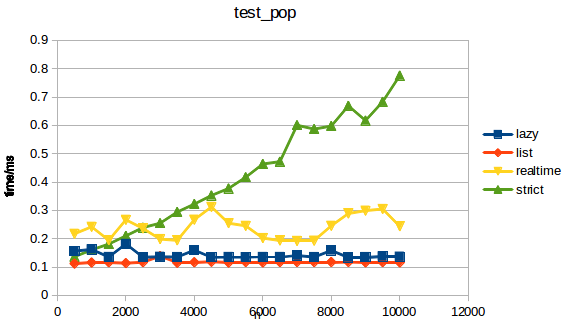
\includegraphics{Graphs/test_pop.png}


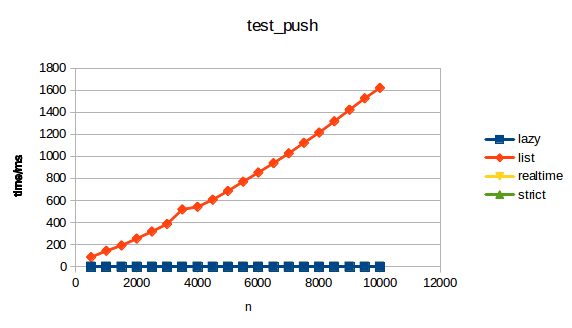
\includegraphics{Graphs/test_push.png}


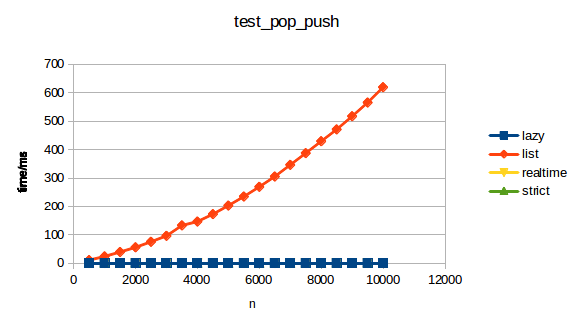
\includegraphics{Graphs/test_pop_push.png}


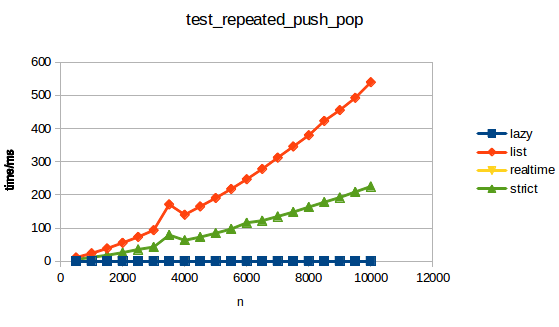
\includegraphics{Graphs/test_repeated_push_pop.png}


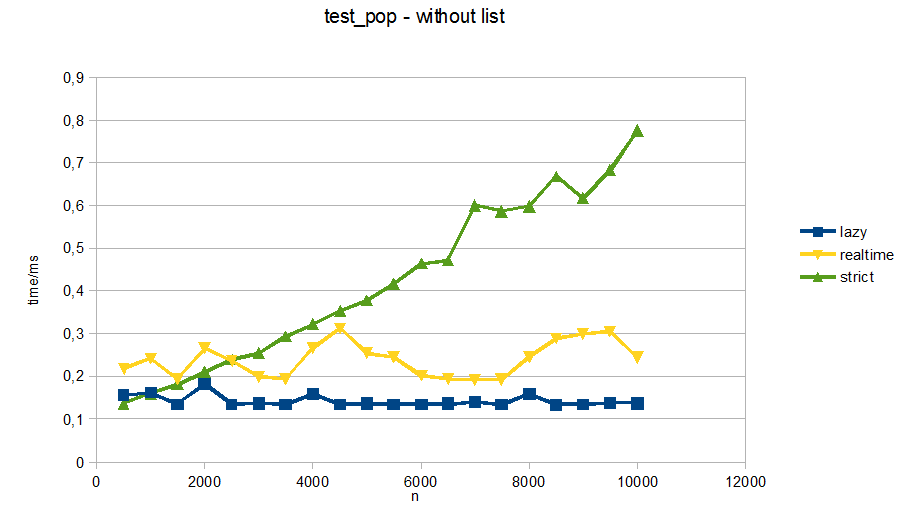
\includegraphics{Graphs/test_pop_without_list.png}


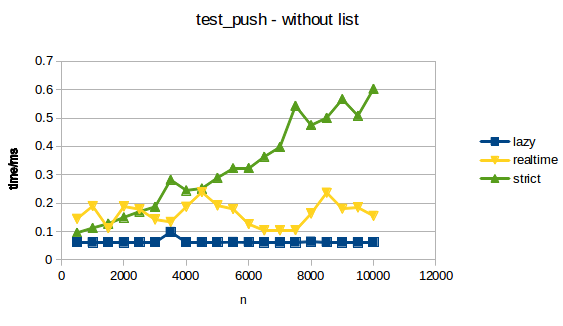
\includegraphics{Graphs/test_push_without_list.png}


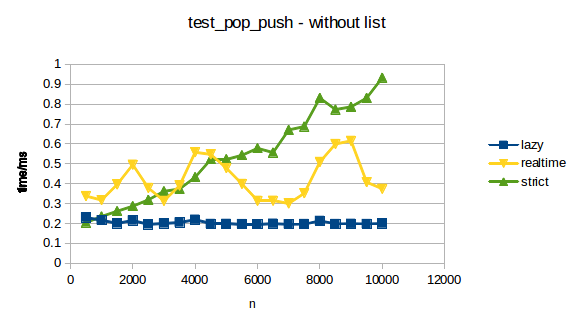
\includegraphics{Graphs/test_pop_push_without_list.png}


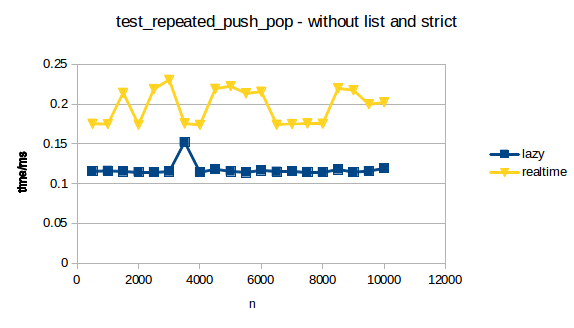
\includegraphics{Graphs/test_repeated_push_pop_without_list.png}


\subsection{Conclusions}
 
 TODO: Write, Kris can easily do this